\documentclass[12pt,fleqn]{exam}
\usepackage{amssymb}
\usepackage[intlimits]{amsmath}
\usepackage{epsfig}
\usepackage{upgreek}
\usepackage[super]{nth}
\usepackage[colorlinks=true,linkcolor=black,anchorcolor=black,citecolor=black,filecolor=black,menucolor=black,runcolor=black,urlcolor=black]{hyperref}
\usepackage[letterpaper, margin=0.75in]{geometry}
\addpoints
\boxedpoints
\pointsinmargin
\pointname{pts}
\usepackage{tikz}
\usepackage{tkz-euclide}
\usetikzlibrary{shapes.geometric}
\usetikzlibrary{calc}
\usepackage[final]{microtype}
\frenchspacing
\usepackage[american]{babel}
\usepackage[T1]{fontenc}
\usepackage[]{fourier}
\usepackage{isomath}
\usepackage{upgreek,amsmath}
\usepackage{graphicx}

\newcommand{\dotprod}{\, {\scriptzcriptztyle\stackrel{\bullet}{{}}}\,}

\newcommand{\reals}{\mathbf{R}}
\newcommand{\lub}{\mathrm{lub}} 
\newcommand{\glb}{\mathrm{glb}} 
\newcommand{\complex}{\mathbf{C}}
\newcommand{\dom}{\mbox{dom}}
\newcommand{\range}{\mbox{range}}
\newcommand{\cover}{{\mathcal C}}
\newcommand{\integers}{\mathbf{Z}}
\newcommand{\vi}{\, \mathbf{i}}
\newcommand{\vj}{\, \mathbf{j}}
\newcommand{\vk}{\, \mathbf{k}}
\newcommand{\bi}{\, \mathbf{i}}
\newcommand{\bj}{\, \mathbf{j}}
\newcommand{\bk}{\, \mathbf{k}}
\DeclareMathOperator{\Arg}{\mathrm{Arg}}
\DeclareMathOperator{\Ln}{\mathrm{Ln}}
\newcommand{\imag}{\, \mathrm{i}}
\newcommand{\erf}{\mathrm{erf}}

\usepackage{graphicx}
\usepackage{color}
%\shadedsolutions
%\definecolor{SolutionColor}{rgb}{1,0.72,0.46} %{0.8,0.9,1}
\newcommand\AM{\textsc{am}}
\newcommand\PM{\textsc{pm}}

\usepackage{array}   % for \newcolumntype macro
\newcolumntype{L}{>{$}l<{$}} % math-mode version of "l" column type
     
\newcommand{\quiz}{23}
\newcommand{\term}{Fall}
\newcommand{\due}{Tuesday 16 April 13:20}
\newcommand{\class}{MATH 202, Spring \the\year}
\begin{document}
\large
\noindent\makebox[3.0truein][l]{\textbf{\class}}
\textbf{Name:} \hrulefill \\
\noindent \makebox[3.0truein][l]{\textbf{In class work  \quiz}}
\textbf{Row and Seat}:\hrulefill\\



\noindent  In class work  \textbf{\quiz}  has questions \textbf{1} 
through  \textbf{\numquestions} \/ with a total of 
\textbf{\numpoints\/} points. Turn in your work at the end of class 
\emph{on paper}. This assignment is due \emph{\due}.

\vspace{0.1in}
\noindent \emph{“There’s no problem so awful that you can’t add some guilt to it and make it even worse.”} \\ \phantom{xxx} \hfill {\sc Calvin (Bill Watterson)}


\begin{questions} 

\question[2] Find the Taylor polynomial of order four centered at zero for the cosine function; that is find the polynomial
$\displaystyle
   P_4(x) = \sum_{k=0}^4 \frac{\cos^{(k)}(0)}{k!} x^k.
$
You'll need to find the numerical values of $\cos^{(0)}(0), \cos^{(1)}(0),  \cos^{(2)}(0),  \cos^{(3)}(0),$ and $ \cos^{(4)}(0)$.
\begin{solution}[3.5in]
Let's make an nicely organized table of derivatives and their values 
at the center; here it is

\begin{center}
\begin{tabular}{| L | L | | L |}
\hline
n & \cos^{(n)}(x) &  \frac{\cos^{(n)}(0)}{n!} \\ \hline 
0 & \cos(x) & 1 \\
1 & -\sin(x) & 0 \\
2 & -\cos(x) & -\frac{1}{2} \\
3 & \sin(x) & 0 \\
4 & \cos(x) & \frac{1}{24} \\ \hline 
\end{tabular}
\end{center}

So $P_4(x) = 1 - \frac{1}{2} x^2 + \frac{1}{24} x^4$.
\end{solution}

\question[2] Use Desmos to graph $y = \cos(x)$ and $y = P_4(x)$, the Taylor polynomial of order four centered at zero for the cosine function.
Reproduce the graph here.  Use the graph to estimate  
maximum of $ \underset{-2 \leq x \leq 2}{\max}| \cos(x) - P_4(x)|$.

\begin{solution}%[2.5in]

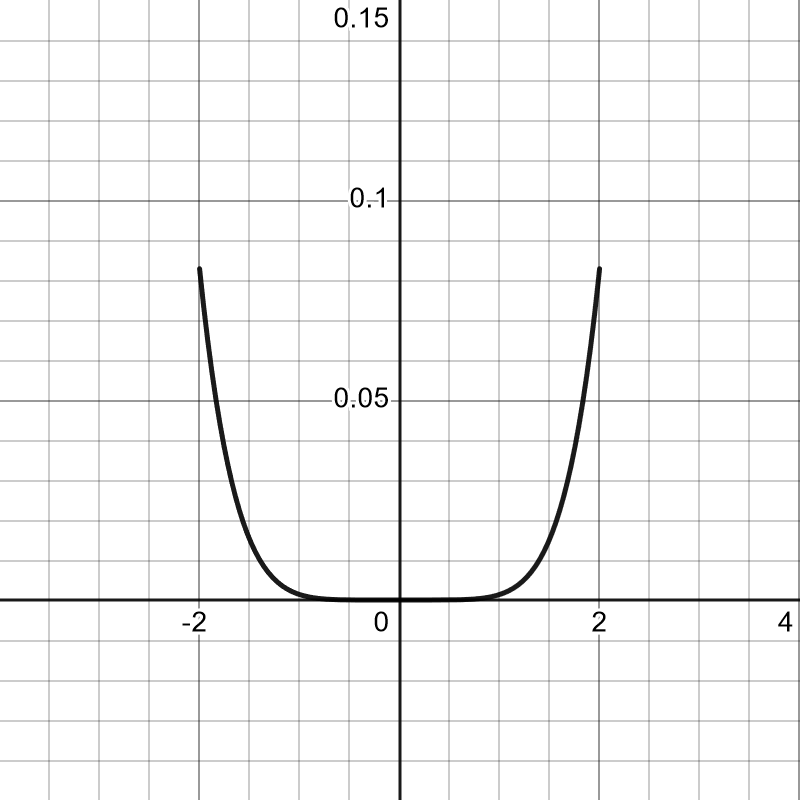
\includegraphics[scale=0.2]{desmos-graph(68).png}

It appears the the maximum difference is about 0.08 (and it occurs at both endpoints).
\end{solution}

\newpage

\question[2] Find the Taylor polynomial of order four centered at zero for the \emph{square} of the cosine function.  You could \emph{suffer}
through the calculation by finding the first four derivatives of $\cos(x)^2$ and evaluate them at zero. Or you could use Cauchy product that we
learned the other day.  The easy way to to this to (a) use your polynomial $P_4$ from Question 1.  Then the Taylor polynomial of order four centered at zero for the \emph{square} of the cosine function
is $P_4(x) P_4(x)$, but when you expand this product, set every power of $x$ that exceeds 4 to zero.


 


\begin{solution}
The easy way to expand $(1 - \frac{1}{2} x^2 + \frac{1}{24} x^4)^2$ and to ignore all powers of $x$ that are degree five
or higher. Thus the 4th order TP for $\cos^2$ centered at zero is
\begin{align*}
   (1 - \frac{1}{2} x^2  + \frac{1}{24} x^4)^2 &= 1 + (-\frac{1}{2} - \frac{1}{2}) x^2 + (\frac{1}{24} + \frac{1}{4} + 
   \frac{1}{24}) x^4 + \text{hot}, \\
      &= 1 - x^2 +  \frac{1}{3} x^4 +  \text{hot}.
\end{align*}
In the physics and engineering communities,  $\text{hot}$ is a context dependent phrase meaning \emph{higher order terms}.
So our TP is $1 - x^2  + \frac{1}{3} x^4 $
\end{solution}

\end{questions}
\end{document}
